% !TeX root = ../Thesis.tex
\documentclass[../Thesis.tex]{subfiles}
\graphicspath{{\subfix{../images/}}}

\begin{document}

\section{Deadlocks}

Deadlocks are a common problem that can occur in concurrent systems,
which are systems where multiple threads or processes are
running simultaneously and potentially sharing resources.
They have been studied at least since \cite{dijkstra1964},
who coined the term ``deadly embrace'' in Dutch, which did not catch on.

A deadlock occurs when two or more threads or processes
are blocked and unable to continue executing
because each is waiting for the other to release a resource that it needs.
This results in a situation where none of the threads or processes
can make progress and the system becomes effectively stuck.

This can be a serious problem in concurrent systems,
as they can cause the system to become unresponsive or even crash.
Therefore, it is important to be able to detect and prevent deadlocks.
They can occur in any concurrent system where multiple threads or processes
are competing for shared resources.
Examples of shared resources that can lead to deadlocks include system memory,
input/output devices, locks, and other types of synchronization primitives.

Deadlocks can be difficult to detect and prevent
because they depend on the precise timing of events in the system.
Even in cases where deadlocks can be detected, resolving them can be difficult,
as it may require releasing resources that have already been acquired or
rolling back completed transactions.
To avoid deadlocks, it is important to carefully manage shared resources in a concurrent system.
This can involve using techniques such as resource allocation algorithms,
deadlock detection algorithms, and other types of synchronization primitives.
By carefully managing shared resources, it is possible to prevent deadlocks from occurring and
ensure the smooth operation of concurrent systems.

To understand the concept in more detail,
consider a simple example where two processes, A and B,
are competing for two resources, X and Y.
Initially, process A has acquired resource X and is waiting to acquire resource Y,
while process B has acquired resource Y and is waiting to acquire resource X.
In this situation, neither process can continue executing
because it is waiting for the other process to release a resource that it needs.
This results in a deadlock, as neither process can make progress.
Fig. \ref{fig:state-graph-example} illustrates this situation.
The cycle therein indicates a deadlock, as will be explained in the section.

\begin{figure}[!htb]
    \centering
    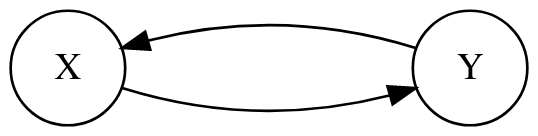
\includegraphics[scale=0.25]{state-graph-example.png}
    \caption{Example of a state graph with a cycle indicating a deadlock.}
    \label{fig:state-graph-example}
\end{figure}
\subsection{Necessary conditions}

According to the classic paper on the topic \cite{coffman1971deadlocks},
the following conditions need to hold for a deadlock to arise.
They are sometimes called ``Coffman conditions''.

\begin{enumerate}
    \item \textbf{Mutual Exclusion}: At least one resource in the system must
          be held in a non-sharable mode, meaning that only one thread or process can use it at a time
          (e.g. a variable behind a mutex).
    \item \textbf{Hold and Wait}: At least one thread or process in the system must
          be holding a resource and waiting to acquire additional resources
          that are currently being held by other threads or processes.
    \item \textbf{No Preemption}: Resources cannot be preempted, which means that a thread or process
          holding a resource cannot be forced to release it until it has completed its task.
    \item \textbf{Circular Wait}: There must be a circular chain of two or more threads or processes,
          where each thread or process is waiting for a resource held by the next one in the chain.
          This is usually visualized in a graph representing the order in which the resources are acquired.
\end{enumerate}

Usually, the first three conditions are characteristics of the system under study, i.e.
the protocols used for acquiring and releasing resources,
while the fourth may or may not occur depending on the interleaving of instructions during the execution.

It is worth noting that the Coffman conditions are in general necessary
but not sufficient for a deadlock to occur.
The conditions are indeed sufficient in the case of single-instance resource systems.
But they only indicate the possibility of deadlock in systems
where there are multiple indistinguishable instances of the same resource.

In the general case, if any one of the conditions is not met, a deadlock cannot occur,
but the presence of all four conditions does not necessarily guarantee a deadlock.
Nonetheless, the Coffman conditions are an important tool for understanding and
analyzing the causes of deadlocks in concurrent systems
and they can help guide the development of strategies for preventing and resolving deadlocks.

\end{document}